\newpage
\section{Appendix: Architecture and Implementation}
\label{app:implementation}

In this section, we describe the neural network architecture and optimization techniques used to parameterize the block-triangular flows.

\subsection{Loss Function and Optimization}

For all models, we use the Adam optimizer \citep{Kingma2015} with a warmup-cosine decay learning rate schedule. This schedule provides an initial linear warmup period followed by a cosine annealing phase to ensure stable convergence.

The training objective for our one-sided flows follows the denoising-style loss for $\eta_1$-prediction:
\begin{equation}
    \mathcal{L}(\theta) = \mathbb{E}_{t \sim \mathcal{U}(0,1), y_1 \sim p_{data}, \epsilon \sim \mathcal{N}(0,I)} \left[ \| \hat{\eta}_1(y_t, t; \theta) - y_1 \|^2 \right]
\end{equation}
where $y_t = t y_1 + (1-t) \epsilon$ is the linear interpolant.

\subsubsection{Noise--Data Coupling}
\label{app:coupling}
\cam{Minibatch optimal transport (OT) couplings, which pair noise samples $\epsilon$ with data samples $y_1$ within each training batch, straighten flow trajectories \citep{tong2023conditional} and so reduce integration error. They preserve the \emph{joint} marginals, but a coupling computed on the full vector $y_1$ is not neutral for \emph{conditionals}: the noise paired with a block then depends on that block's conditions, so the population optimum of the flow-matching loss no longer transports to the correct conditional distributions \citep{cheng2025curse}. Which coupling is admissible therefore depends on the conditioning mode:
\begin{itemize}
    \item \textbf{Static:} independent pairing ($\epsilon \perp y_1$). Each block's network receives its conditions as clean inputs, and independent pairing is exact for every conditional.
    \item \textbf{Dynamic:} a per-block coupling in topological order. Each block's noise is matched to its data within the batch by a condition-aware OT plan \citep{cheng2025curse} whose cost adds the parents' squared distance with a weight chosen per batch by the adaptive rule of \citet{cheng2025curse}: the smallest weight for which at most $5\%$ of pairs $(i,j)$ have a combined cost below that of the unpermuted pair $(i,i)$. This is a minibatch Knothe--Rosenblatt coupling. Unlike independent pairing, this makes the marginal velocity of each block depend only on the block and its predecessors, which a block-triangular field can represent (Remark~\ref{rem:dynamic-consistency}).
    \item \textbf{Guided:} exact minibatch OT (Hungarian) on the joint vector; the guided flow models the joint, which this coupling preserves.
\end{itemize}

\paragraph{Population limit of the minibatch coupling on chains.} A batch-$128$ matching only approximates the Knothe--Rosenblatt coupling, so even at the optimum it leaves some bias. For the linear-Gaussian chains of Section~\ref{sec:chain-stiffness} this residual can be computed without training. We apply the training coupling to $300$ batches of $128$ standardized samples and take the empirical cross-covariance $C = \mathrm{Cov}(\epsilon, y_1)$. Treating $(\epsilon, y_1)$ as jointly Gaussian with that covariance, the best block-triangular field is linear: row $k$ is the regression of $\dot y^{(k)} = y_1^{(k)} - \epsilon^{(k)}$ on $y_t^{(1:k)}$. We integrate the induced covariance ODE from $\mathcal{N}(0, I)$ and compare $p(x_0 \mid x_{n-1})$ with the exact posterior in $W_2$. With the exact Knothe--Rosenblatt coupling (Cholesky) this gives $0$, and with independent pairing it matches the trained dynamic models to within $0.11$ at every depth. With the minibatch coupling it gives $0.009$, $0.012$, $0.028$, $0.053$ and $0.075$ for $n = 2, \dots, 32$. Each block's matched noise has correlation ${\approx}0.65$ with its exact Knothe--Rosenblatt noise at every depth: the per-block approximation does not degrade with depth, but its residual accumulates along the chain.}

\subsection{Neural Network Architecture}

For each variable in the PGM, we use a conditional block which computes the output (the velocity, or the prediction $\hat\eta_1$ of the clean data) of that variable given its current state $y_t$, the time $t$, and the values of its parent variables $\{p_i\}$ in the dependency graph.

\subsubsection{Residual Block Architecture}
Across all our conditional blocks and networks, we employ a consistent architecture based on residual layers. The key design is:
\begin{itemize}
    \item \textbf{Time Embedding:} The scalar time $t$ is embedded into a high-dimensional vector using Fourier features (random Gaussian projection followed by sin/cos transformations).
    \item \textbf{Input Projection:} The concatenated input (local state, time embedding, and parent states) is projected to a hidden dimension.
    \item \textbf{Residual Stack:} A stack of 8 residual layers, where each layer computes $h \gets h + \sigma(\text{Linear}(\text{LayerNorm}(h)))$. We use Layer Normalization \citep{Ba2016} and the Swish (SiLU) activation function \citep{Ramachandran2017, Elfwing2018} consistently throughout.
    \item \textbf{Output Projection:} A final linear layer projects the hidden representation to the target dimension.
\end{itemize}
This modular residual design is used consistently across all network variants (static conditioning, guidance, CAREFL conditioning, and parallel flows).

To further ensure comparability of the varying architectures (e.g., a single large joint flow versus many small conditional blocks), we adopt a parameter-budgeting approach. For a given budget (e.g., 100,000 parameters), we perform a search over the hidden width $W$ such that the total number of trainable weights in the architecture most closely matches the budget.

\subsection{Structured Flows}

We verify that our models have the intended structure; an example is shown in Figure~\ref{fig:extraction-visualization}.

\begin{figure}[hbt!]
    \centering
    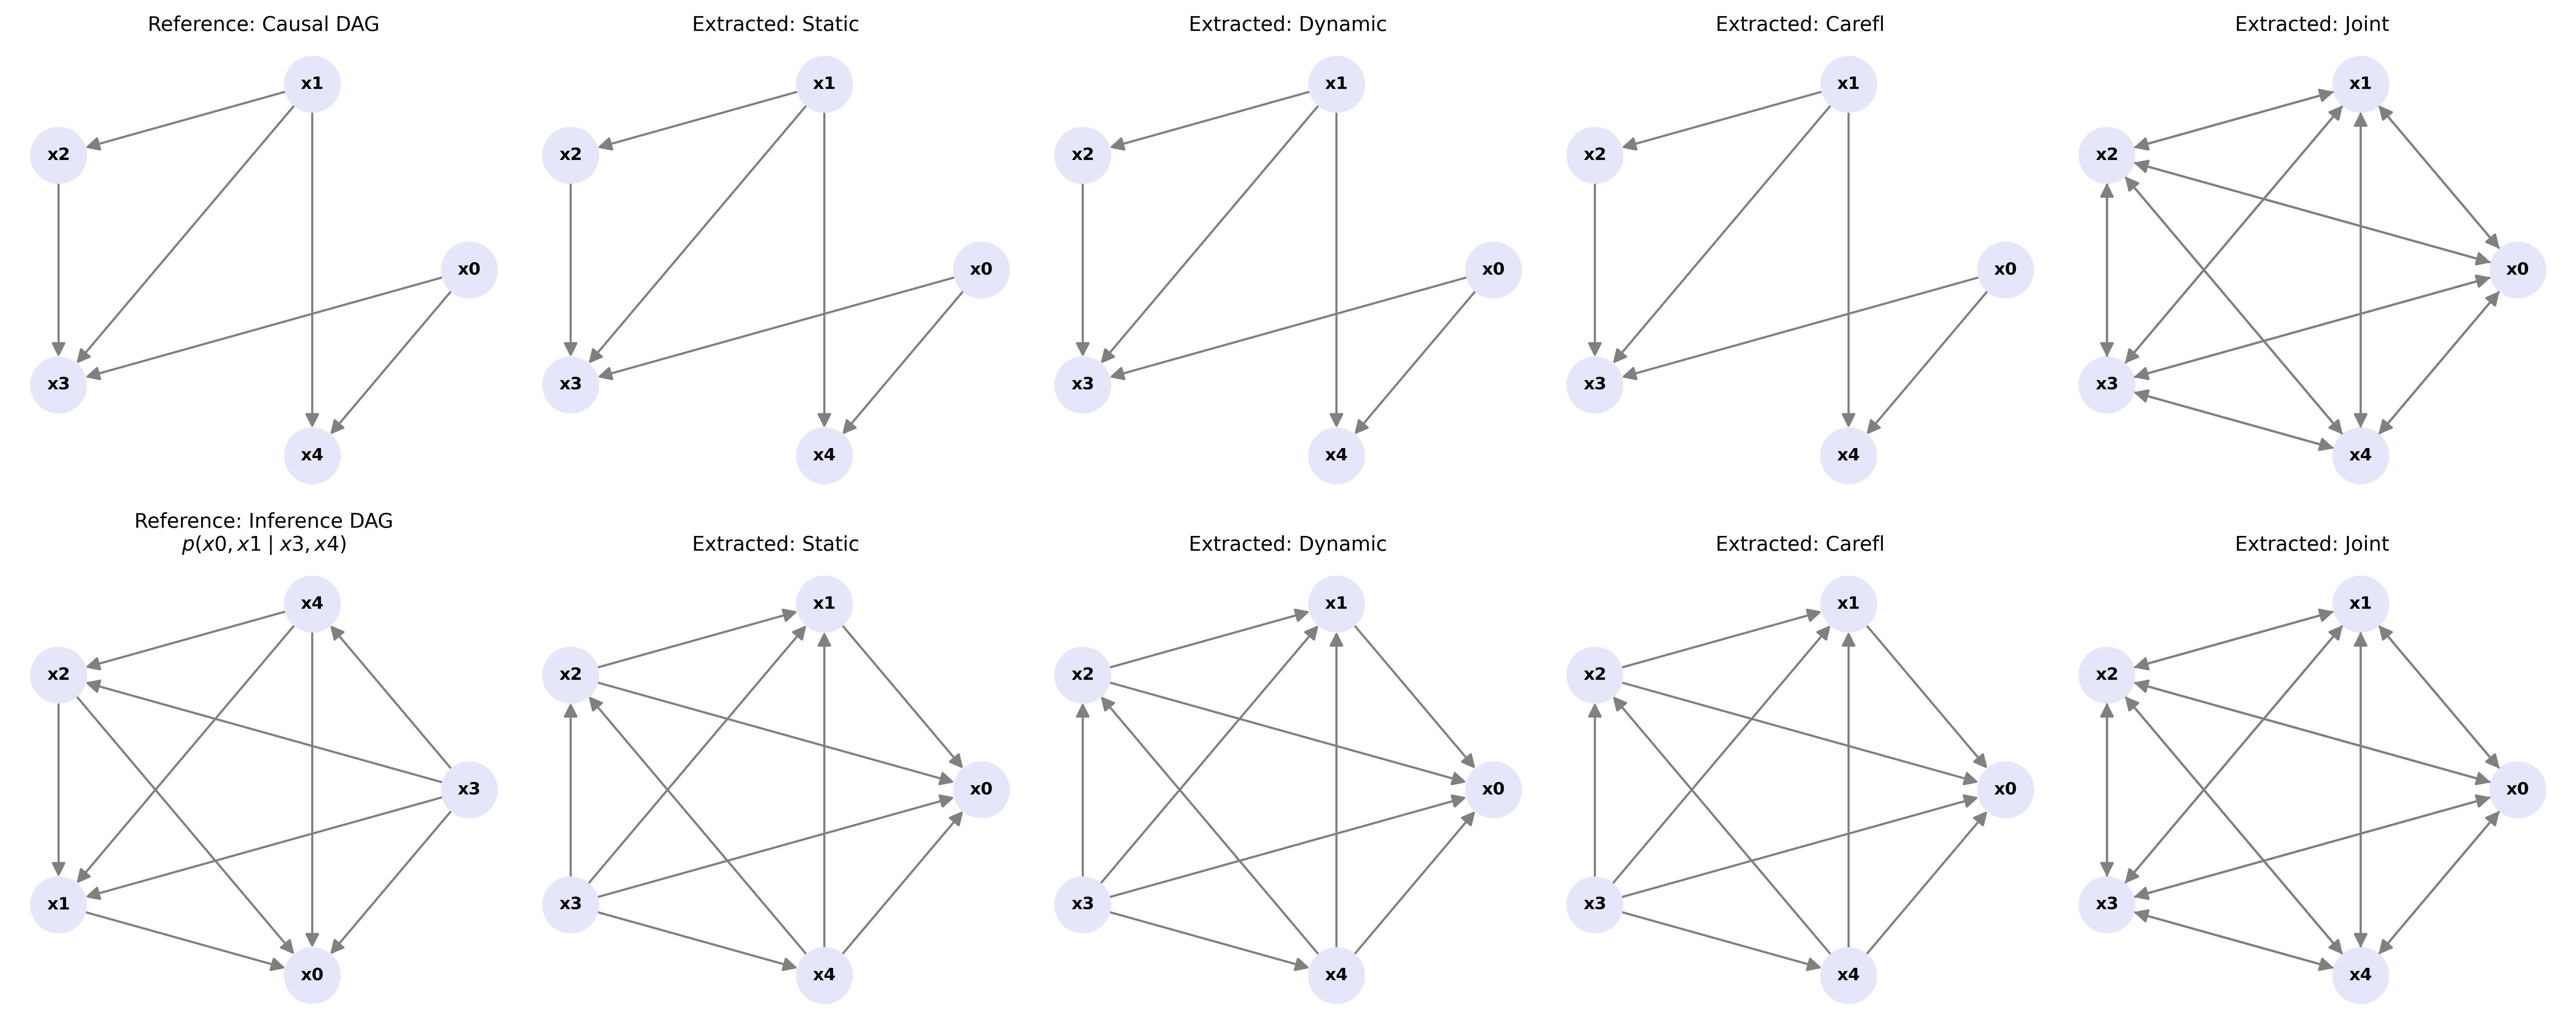
\includegraphics[width=\columnwidth]{images/pgm_compilation_and_extraction_visualization_42.png}
    \caption{Given a PGM, we extract its DAG. The DAG is either used directly as the structure of a causal flow, or compiled into an inference-aligned DAG from which an inference flow is built.}
    \label{fig:extraction-visualization}
\end{figure}
